\documentclass[11pt]{article}

\usepackage[margin=1in]{geometry}
\usepackage{amsmath,amssymb,mathtools,bm}
\usepackage{graphicx}
\usepackage{booktabs}
\usepackage{placeins}
\usepackage[colorlinks=true,linkcolor=blue,citecolor=blue,urlcolor=blue]{hyperref}

\graphicspath{{../figs/}}

% --- macros (shared with the companion analytic paper) ---
\newcommand{\rs}{\bm{r}_s}
\newcommand{\rw}{\bm{r}_w}
\newcommand{\Del}{\bm{\Delta}}
\newcommand{\nhat}{\hat{\bm{n}}}
\newcommand{\uhat}{\hat{\bm{u}}}
\newcommand{\Bhat}{\hat{\bm{B}}}
\newcommand{\Nfp}{N_{\mathrm{fp}}}
\newcommand{\eps}{\varepsilon}
\newcommand{\epseff}{\eps_{\mathrm{eff}}}
\newcommand{\half}{\tfrac{1}{2}}
\newcommand{\NWL}{\mathrm{NWL}}
\newcommand{\dd}{\,\mathrm{d}}
\newcommand{\iso}{\mathrm{iso}}

\title{\bfseries A Monte-Carlo Spin-Polarized Fusion Neutron Source for Stellarator
Wall-Loading, and its Cross-Validation Against the Analytic Field-Period Method}

\author{
Thaddaeus Kiker\textsuperscript{1,2}
\and
Ethan Peterson\textsuperscript{3}
\\[4pt]
\small \textsuperscript{1}Department of Astronomy, Columbia University, New York, NY, USA\\
\small \textsuperscript{2}Fusion Research Center, Columbia University, New York, NY, USA\\
\small \textsuperscript{3}Plasma Science and Fusion Center, Massachusetts Institute of Technology, Cambridge, MA, USA
}
\date{\today}

\begin{document}
\maketitle

\begin{abstract}
\noindent
Spin polarization of deuterium--tritium fuel both enhances the fusion rate and makes the
$14.1$~MeV neutron emission anisotropic about the local magnetic field, so the first-wall
neutron load of a polarized reactor depends on the plasma shape, the field geometry, and
the polarization mix together. A companion paper reduces this load to closed,
differentiable form for weakly shaped quasi-axisymmetric (QA) stellarators by a
field-period perturbation, valid while the geometric non-axisymmetry is small. Here we
build the complementary tool: a Monte-Carlo spin-polarized fusion neutron \emph{source}
for OpenMC that samples the polarized birth direction exactly for an arbitrary
polarization mix and arbitrary local field, carries no restriction on the plasma shaping,
and, unlike the analytic method, ray-traces the true device geometry and admits neutron
transport (scattering) on a realistic first wall. We give the emission kernel and its
separation into a birth-direction distribution and a scalar rate factor, an exact
stratified sampler for the two polarized angular shapes with a closed-form inverse-CDF
cross-checked against rejection, and a robust local$\to$global frame rotation. We verify
the sampler in isolation---the sampled directionality reproduces the normalized kernels
to $0.3\%$ per bin with unit mean---and then cross-validate the full source against the
analytic method in the free-streaming limit where the two must agree. On a gentle toy QA
boundary ($\epseff\!\approx\!0.08$) the two methods agree to $\le1.8\%$ on all four walls
of a square-cross-section torus; on a real, published QA equilibrium mined from the QUASR
database ($\epseff\!\approx\!0.43$) they agree to $\le1.8\%$ on three walls, with a
$4$--$6\%$ residual isolated to the inner (inboard) wall. We show, by elimination and by
a direct single-filament construction, that this residual is a limit of the analytic
point-patch flux integral on a strongly curved wall under strong shaping---exact for an
axisymmetric source and growing as the square of the shaping amplitude---and not a defect
of the Monte-Carlo source, whose sampler, geometry, and transport are exact. The result
delineates the division of labour between the two methods: the closed form for weakly
shaped QA where gradients are cheap, and the present source for strongly shaped
geometries and for the scattering problem that the free-streaming analytic cannot
address.
\end{abstract}

\section{Introduction}
\label{sec:intro}

Spin-polarized fusion (SPF) aligns the reactant nuclear spins to raise the D--T reaction
cross section by up to $50\%$ and to redirect the angular distribution of the fusion
products~\cite{kulsrud1982,parisi2024,schwartz2025}. The neutron carries $80\%$ of the
D--T energy, so the redistribution of the $14.1$~MeV neutrons directly reshapes the
first-wall neutron load---the quantity that sets the blanket, shield, and material
lifetimes of a reactor---and the optimal polarization choice is a system decision that
must be made against that load~\cite{schwartz2025,lion2022}. Scoping studies quantify the
load through the neutron wall load (NWL), the first-flight neutron current through a wall
patch weighted by the neutron energy; it omits scattering but is inexpensive and is
therefore the natural object for design iteration~\cite{lion2022,schwartz2025}.

The polarized neutron emission is not isotropic. For a chosen mixture of deuteron and
triton spin projections the differential cross section is a fixed combination of two
angular shapes referred to the local field direction $\Bhat$: a $\sin^2\theta$ shape that
peaks perpendicular to $\Bhat$ and a $\tfrac14+\tfrac34\cos^2\theta$ shape that peaks
parallel to it, where $\theta$ is the angle between the emitted neutron and
$\Bhat$~\cite{schwartz2025}. Because $\Bhat$ follows the magnetic geometry, the wall load
of a polarized plasma is a convolution of the emission kernel, the field, and the source
distribution over the plasma volume against the wall geometry.

Two complementary routes evaluate this convolution. The first is analytic. For an
axisymmetric device the toroidal source integral over a planar ring reduces to incomplete
elliptic integrals, giving a fast, automatically differentiable NWL suited to shape and
polarization optimization~\cite{schwartz2025}. A stellarator source loop is non-planar,
the period integral becomes hyperelliptic, and the closed form is lost; the companion
paper restores it perturbatively for weakly shaped QA boundaries by expanding in the
geometric non-axisymmetry, with a single-quadrature fallback where the expansion is slow.
That method is powerful precisely where its controlling parameter---the geometric
excursion of the boundary relative to the wall standoff, $\epseff$---is small, and it is a
free-streaming (uncollided) method by construction.

The second route, developed here, is Monte-Carlo. We build an SPF neutron source for
OpenMC~\cite{romano2015}: given a polarization mix, a birth position distribution over the
plasma, and the local field, it samples the polarized birth direction and hands OpenMC a
neutron that is then transported through the true device geometry. This route makes no
assumption about the magnitude of the shaping, ray-traces the exact walls rather than
approximating each patch as a point, and---its decisive advantage---admits full neutron
transport, so the same source that reproduces the free-streaming NWL can be run with
scattering on a CAD or constructive-solid-geometry (CSG) first wall to obtain the actual
volumetric loads that a reactor blanket sees. The two methods are therefore not
competitors but a division of labour: closed-form gradients where the boundary is weakly
shaped, and the Monte-Carlo source where it is strongly shaped or where transport matters.

A Monte-Carlo source is only useful if it is demonstrably correct, and the natural check
is that it reproduces the analytic NWL in the regime where the analytic method is itself
exact---the free-streaming limit at small $\epseff$. This paper is organized around that
check and its one interesting failure. Section~\ref{sec:source} states the emission kernel
and separates it into a birth-direction distribution and a scalar rate factor.
Section~\ref{sec:mc} gives the exact stratified direction sampler, the birth-position and
field models, and the OpenMC realization. Section~\ref{sec:sampler} verifies the sampler
in isolation. Section~\ref{sec:validation} cross-validates the full source against the
analytic method on a toy QA boundary and on a real published QA equilibrium.
Section~\ref{sec:pointpatch} isolates the one residual---on the strongly curved inboard
wall of the strongly shaped case---and shows, by elimination and by direct construction,
that it is a limit of the analytic point-patch flux integral and not of the Monte-Carlo
source. Section~\ref{sec:outlook} describes the transition to the transport problem, and
Section~\ref{sec:summary} summarizes.

\section{The spin-polarized emission source}
\label{sec:source}

We follow the parameterization of Ref.~\cite{schwartz2025}. Let the deuteron spin
projection fractions be $d_+,d_0,d_-$ and the triton fractions $t_+,t_-$. The three
collision-mode fractions are
\begin{equation}
a=d_+t_++d_-t_-,\qquad b=d_0,\qquad c=d_+t_-+d_-t_+,\qquad a+b+c=1,
\label{eq:abc}
\end{equation}
with the unpolarized fuel at $a=b=c=\tfrac13$. The differential cross section, referred to
the local field direction $\Bhat$, is
\begin{equation}
\frac{\dd\sigma}{\dd\Omega}=\frac{\sigma_0}{2\pi}\left[\tfrac34\,a\,\sin^2\theta
+\left(\tfrac23 b+\tfrac13 c\right)\left(\tfrac14+\tfrac34\cos^2\theta\right)\right],
\qquad \cos\theta=\Bhat\cdot\hat{\bm\Delta},
\label{eq:dsdo}
\end{equation}
where $\hat{\bm\Delta}$ is the emitted neutron direction and $\sigma_0$ is the cross
section in the $S=\tfrac32$ combined-spin state. Integrating Eq.~\eqref{eq:dsdo} over the
sphere gives the total rate $\sigma_{\rm tot}=\sigma_0\,\eta$ with
$\eta=a+\tfrac23 b+\tfrac13 c$; the unpolarized value is $\tfrac23\sigma_0$, pure $a$
(mode A) is $\sigma_0$ (a $50\%$ enhancement), and pure $c$ (mode C) is $\tfrac13\sigma_0$.
Modes B and C share the same angular shape $\tfrac14+\tfrac34\cos^2\theta$ and differ only
in rate: the emission of a polarized plasma is controlled by two angular functions, not
three.

The essential structure for sampling is that the \emph{birth direction} and the
\emph{total rate} separate. Collecting the two angular shapes,
\begin{equation}
I(\theta)=w_\perp\sin^2\theta+w_\parallel\!\left(\tfrac14+\tfrac34\cos^2\theta\right),
\qquad w_\perp=\tfrac34 a,\quad w_\parallel=\tfrac23 b+\tfrac13 c,
\label{eq:I}
\end{equation}
the normalized birth-direction density is $p(\theta,\phi)=I(\theta)/\!\int I\dd\Omega$ with
$\phi$ uniform, and it depends only on $(w_\perp,w_\parallel)$. The overall rate factor
$\eta$ multiplies the spatial source strength and does not enter the direction sampling.
Keeping these two concerns separate is the central design choice: the sampler draws a
correctly shaped direction for any $(a,b,c)$, and $\eta$ is applied, if absolute loads are
wanted, as a scalar weight on the birth-position distribution. For the free-streaming
cross-checks of this paper the direction is all that matters, and the birth energy is
taken monoenergetic at $14.1$~MeV; a Ballabio-broadened Gaussian at a specified ion
temperature is available for physical runs and is irrelevant to the angular
verification.

\section{Monte-Carlo realization}
\label{sec:mc}

\paragraph{Exact stratified direction sampling.}
Because Eq.~\eqref{eq:I} is a nonnegative combination of two shapes, we sample the birth
direction by stratification: with probability $W_\perp/(W_\perp+W_\parallel)$ draw from
the $\sin^2\theta$ shape, otherwise from the $\tfrac14+\tfrac34\cos^2\theta$ shape, where
$W_\perp=w_\perp\!\int\!\sin^2\theta\dd\Omega=\tfrac{8\pi}{3}w_\perp$ and
$W_\parallel=w_\parallel\!\int(\tfrac14+\tfrac34\cos^2\theta)\dd\Omega=2\pi w_\parallel$
are the solid-angle-integrated weights. This is an exact draw from the mixture and makes
per-mode verification trivial. Each shape is sampled by a closed-form inverse-CDF in
$x=\cos\theta$: the $\sin^2\theta$ shape has marginal $\propto\sin^3\theta$ and is inverted
by the trigonometric solution of the depressed cubic $x^3-3x+2(1-2\xi)=0$; the
$\tfrac14+\tfrac34\cos^2\theta$ shape has marginal $\propto\tfrac14+\tfrac34x^2$ and is a
cubic in $x$ as well. Each inverse-CDF is cross-checked against an independent rejection
sampler (envelope $\propto\sin\theta$, acceptance $\tfrac23$) to a two-sample
Kolmogorov--Smirnov tolerance, so the root selection in the cubic is verified rather than
assumed. The azimuth $\phi$ is uniform on $[0,2\pi)$.

\paragraph{Local-to-global rotation.}
The sampled direction is expressed in a frame with $\hat{\bm z}_{\rm loc}\parallel\Bhat$
and rotated to global Cartesian by a Gram--Schmidt construction that avoids the
$\Bhat\parallel\hat{\bm z}$ degeneracy: the reference axis is whichever of
$\hat{\bm x},\hat{\bm y},\hat{\bm z}$ is least aligned with $\Bhat$, and
$\hat{\bm x}_{\rm loc}=\mathrm{normalize}(\hat{\bm e}_{\rm ref}-(\hat{\bm e}_{\rm ref}\!\cdot\!\Bhat)\Bhat)$,
$\hat{\bm y}_{\rm loc}=\Bhat\times\hat{\bm x}_{\rm loc}$. The resulting global direction is
unit to machine precision and, tested with a random non-axis $\Bhat$, leaves an isotropic
local distribution isotropic---the check that the rotation carries no bias.

\paragraph{Birth positions and field.}
The birth-position model is pluggable. For the cross-checks the plasma is represented by
constant-$(\rho,\vartheta)$ filaments on a set of scaled flux surfaces, sampled uniformly
in the toroidal angle and weighted by the arc-length Jacobian and a model emissivity
$W(\rho)\propto\rho^2$; the same filaments are the source loops of the analytic method, so
the two calculations share the source exactly and the comparison isolates the transport
treatment. The local field direction $\Bhat$ is evaluated at each birth point. For the
real-equilibrium test we take the flux-surface-tangent field
$\Bhat\propto\partial_\phi\bm r+\iota\,\partial_\vartheta\bm r$ at the device rotational
transform $\iota$, i.e.\ the field-line direction implied by the boundary geometry and the
transform; because both the analytic and the Monte-Carlo evaluation call the identical
$\Bhat$, the comparison is valid independent of how faithfully this model reproduces the
true equilibrium field.

\paragraph{OpenMC source and transport.}
The sampled births are handed to OpenMC~\cite{romano2015} either through a compiled
custom-source shared library or, as used here, as a pre-sampled source bank written to an
HDF5 file and read back as a fixed source. For the free-streaming cross-checks the vessel
interior is void and the walls are vacuum boundaries, so each neutron streams in a
straight line from its birth point until it crosses a surface and is tallied; the wall
load is a surface-current tally binned poloidally. This ray-traced transport makes no
point-patch or $1/D^2$ approximation---a neutron reaches a wall patch if and only if its
sampled trajectory does---which is the property that the analytic comparison below tests.
The same source, run with a material first wall and blanket rather than a void, gives the
transported load; that calculation is the subject of Sec.~\ref{sec:outlook}.

\section{Verification of the sampler}
\label{sec:sampler}

The sampler is verified before any geometry is introduced. Drawing $2\times10^6$
directions per mode about a fixed $\Bhat=\hat{\bm z}$ and histogramming in equal
$\cos\theta$ bins, the sampled directionality---the ratio of the mode density to the
isotropic density in each bin---reproduces the normalized kernels
$\tfrac32\sin^2\theta$ (mode A) and $2(\tfrac14+\tfrac34\cos^2\theta)$ (mode B/C) to
better than $0.3\%$ per bin, and the mean directionality of each polarized mode is
$1.0000$, confirming that the stratified draw is normalized to unit emission exactly
(Table~\ref{tab:sampler}). A $\chi^2$ test against the analytic $p(\cos\theta)$ for
$\{$unpolarized, A, B, C, mixed$\}$ and a two-sample KS test of inverse-CDF against
rejection close the sampler verification; the isotropic and rotation-isotropy checks are
flat as required. This isolates the sampler from every subsequent test: any later
discrepancy is geometric, not a defect of the angular draw.

\begin{table}[t]
\centering
\caption{Sampler self-test: sampled directionality $A/\iso$ and $B/\iso$ per
$\cos\theta$ bin against the exact normalized kernels, and the mode means. The sampled
kernels match to $0.3\%$ and integrate to unit emission ($1.0000$), so the direction draw
is exact independent of any geometry.}
\label{tab:sampler}
\begin{tabular}{cccccc}
\toprule
$\cos\theta$ & $A/\iso$ (MC) & $\tfrac32\sin^2\theta$ & $B/\iso$ (MC) & $2(\tfrac14+\tfrac34\cos^2\theta)$ \\
\midrule
$-0.95$ & $0.146$ & $0.146$ & $1.857$ & $1.854$ \\
$-0.15$ & $1.467$ & $1.466$ & $0.535$ & $0.534$ \\
$+0.05$ & $1.491$ & $1.496$ & $0.505$ & $0.504$ \\
$+0.85$ & $0.414$ & $0.416$ & $1.582$ & $1.584$ \\
\midrule
mean & $1.0000$ & $1$ & $1.0000$ & $1$ \\
\bottomrule
\end{tabular}
\end{table}

\section{Cross-validation against the analytic method}
\label{sec:validation}

The decisive test is that the Monte-Carlo source reproduces the analytic free-streaming
NWL where the analytic method is itself exact. We compare on a shared square-cross-section
torus wall, so that all non-axisymmetry lives in the source and the wall is common to both
calculations, and we compare the wall directionality $A/\iso$ and $B/\iso$---the ratio of
the polarized load to the isotropic load on each wall---which cancels the source
normalization and isolates the polarized steering. The analytic side is a pure-numpy
free-streaming quadrature that evaluates the loop geometry and field directly at the
Gauss--Legendre nodes with the true shaped-loop visibility and the inner-cylinder
occlusion; it is gated at run time against the companion \texttt{anarr\'ima} quadrature
and matches it to $10^{-12}$, so it is the analytic method's own reference, only faster.

\paragraph{A gentle toy QA boundary.}
The first case is a deliberately gentle QA boundary with $\Nfp=2$, unit major radius,
minor radius $\approx0.17$, and small non-axisymmetric harmonics giving a gently
rotating-elliptical cross section, at $\epseff\approx0.08$. The source is filaments on two
scaled flux surfaces with a $\rho^2$ emissivity and a model field carrying a mean pitch
and a field-period ripple; the wall is the square torus at a fixed gap. With $10^6$
births per mode the Monte-Carlo directionality matches the analytic on all four walls to
$\le1.8\%$ (Table~\ref{tab:toy}), and the per-bin poloidal profiles track---the
correlation between the Monte-Carlo and analytic $A/\iso$ profiles is $0.85$--$0.98$ on
the walls that carry a poloidal gradient (Fig.~\ref{fig:toy}). The gentle case therefore
validates the whole chain---sampler, birth model, field, ray-traced transport, and
tally---against the analytic method with no residual beyond Monte-Carlo statistics.

\begin{figure}[t]
\centering
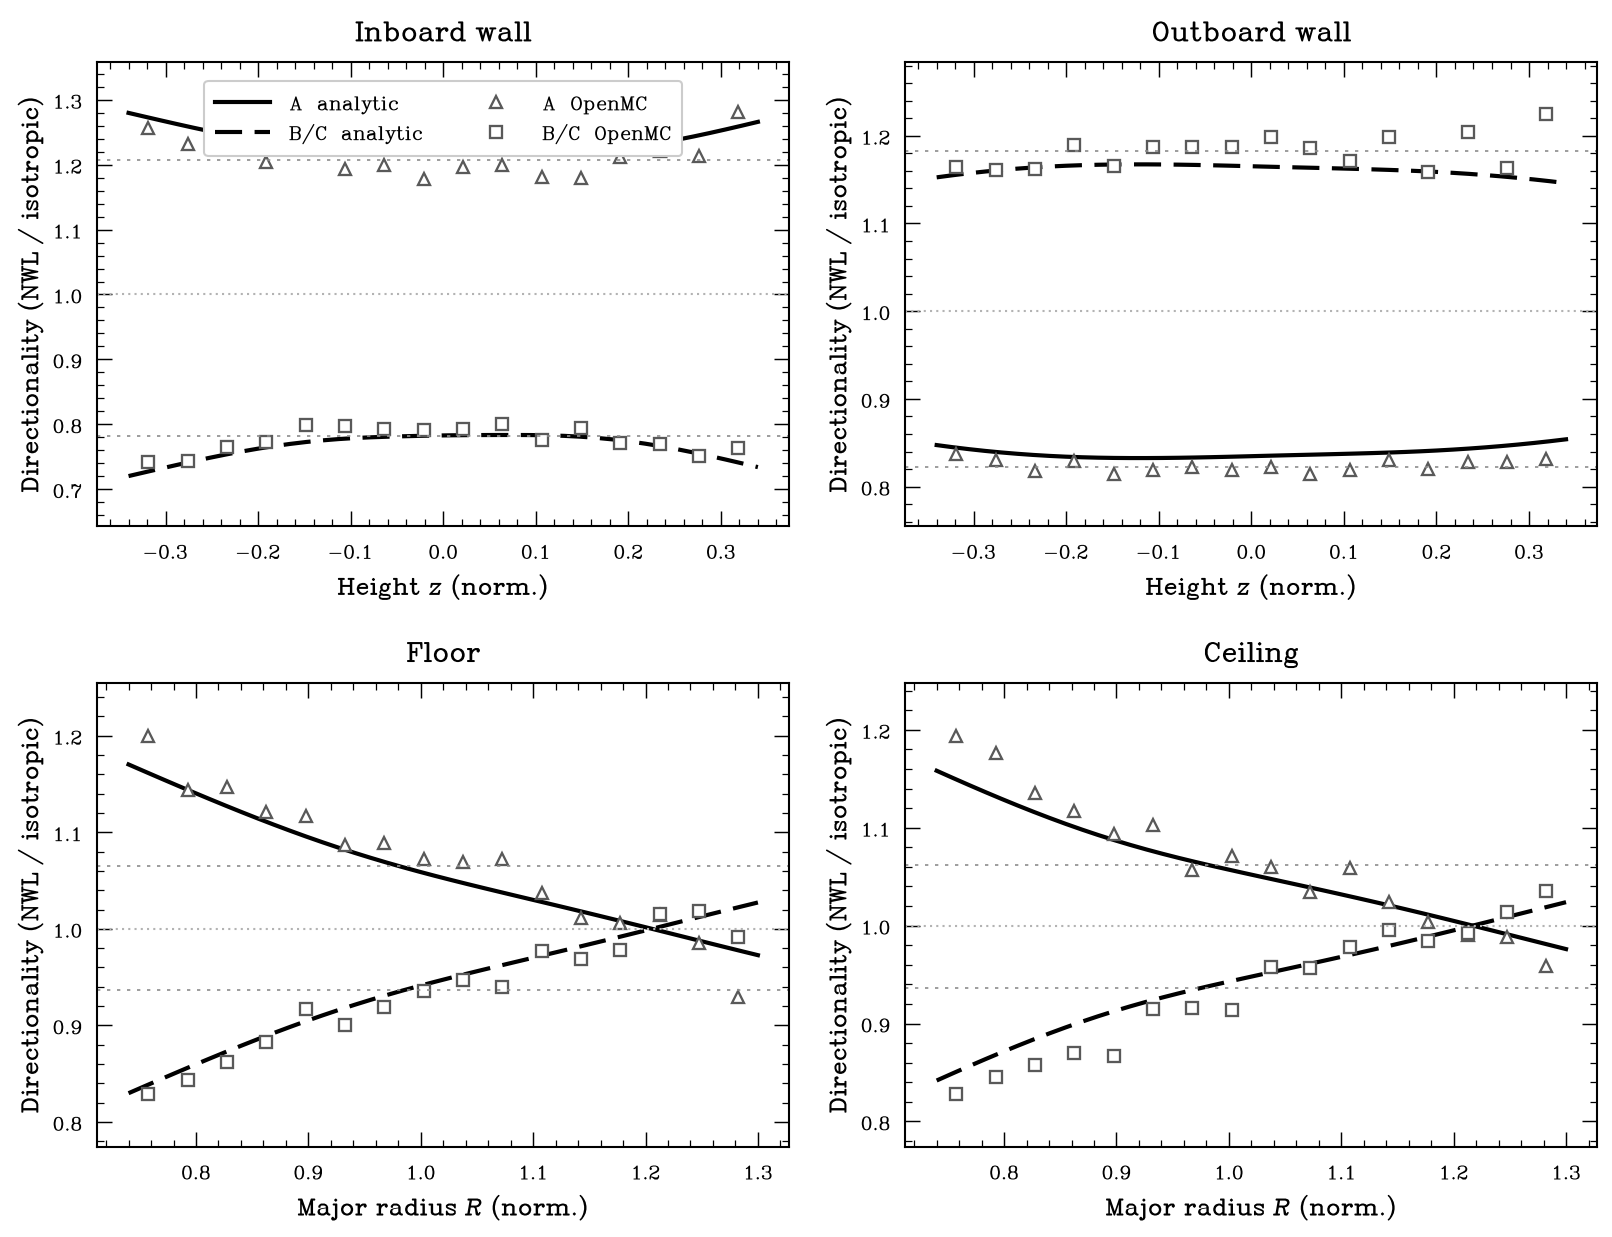
\includegraphics[width=\linewidth]{toy_qalow_directionality.png}
\caption{Free-streaming directionality on the gentle toy QA boundary
($\epseff\approx0.08$): analytic point-patch flux integral (curves) and OpenMC
ray-traced source (markers) for modes A and B/C around each wall of the square torus. All
four walls overlay to $\le1.8\%$; the poloidal profiles track to correlation
$0.85$--$0.98$ on the walls that carry a gradient.}
\label{fig:toy}
\end{figure}

\paragraph{A real, published QA equilibrium.}
The second case uses a genuine published equilibrium. Because the standard published QA
configurations are all strongly shaped---a survey of DESC examples gives $\epseff\approx
1$--$2.6$ at a tight wall---we mined the QUASR stellarator database~\cite{quasr} for a
gentle one without the bulk download, by pulling its single tabulated catalogue
($3.7\times10^5$ devices), filtering to quasi-axisymmetry ($7.2\times10^4$ devices),
ranking by a metadata proxy that correlates with the geometric excursion (correlation
$0.94$), and computing the exact $\epseff$ of a shortlist from their VMEC boundary
spectra. The gentlest is a $\Nfp=3$ QA of aspect ratio $6.7$ (unit major radius, minor
radius $\approx0.175$), which at the validation wall has $\epseff\approx0.43$---four times
more shaped than the toy and, unlike the toy, near the edge of the analytic method's
convergent band. Its rotating cross section is shown in Fig.~\ref{fig:quasrgeom}.

\begin{figure}[t]
\centering
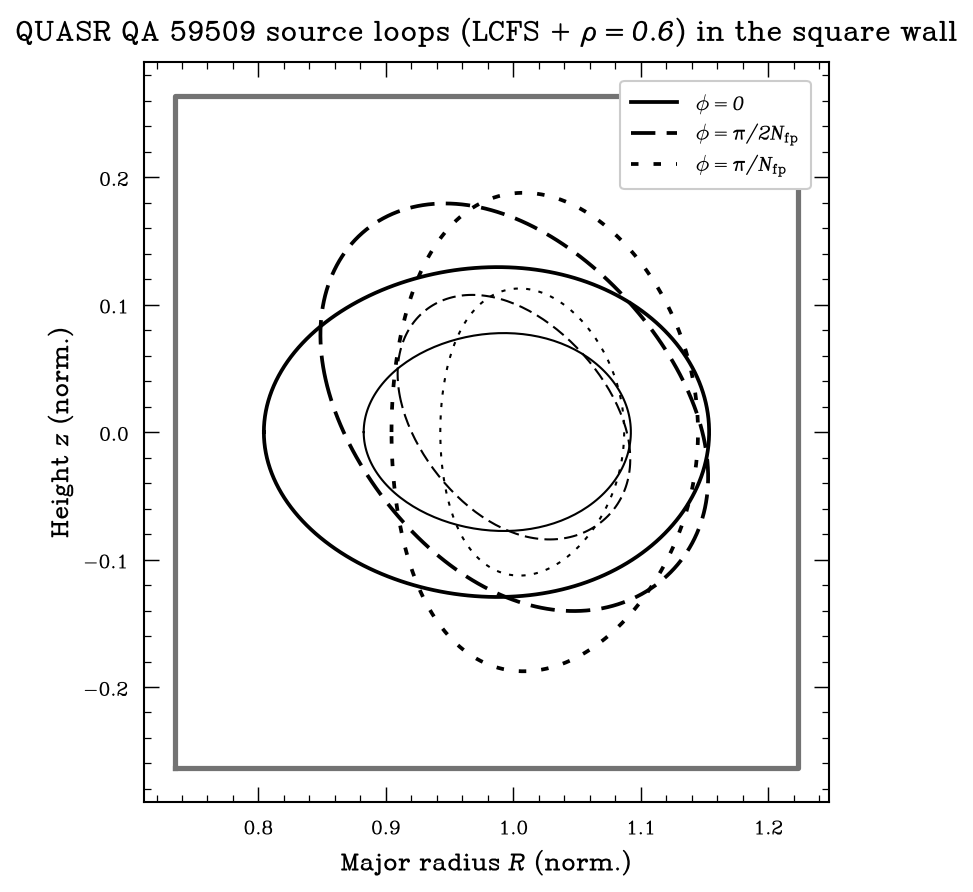
\includegraphics[width=0.62\linewidth]{quasr59509_geometry.png}
\caption{Source loops of the real QUASR QA equilibrium (device 59509, $\Nfp=3$): the
last-closed and an interior flux surface at several toroidal cuts, showing the rotating,
strongly shaped cross section, inside the square-cross-section wall used for the
cross-check.}
\label{fig:quasrgeom}
\end{figure}

On this configuration the Monte-Carlo and analytic directionalities agree to $\le1.8\%$ on
the outboard, floor, and ceiling walls, with the poloidal profiles tracked to correlation
$0.7$--$0.99$; the inner (inboard) wall shows a larger, $4$--$6\%$ residual
(Table~\ref{tab:quasr}, Fig.~\ref{fig:quasr}). The inboard wall is where the analytic
companion paper's own controlling parameter $\epseff$ is largest---it is local and peaks
where the standoff is smallest---so a departure there, on the most strongly curved wall of
the most strongly shaped case, is exactly where one expects the free-streaming analytic to
be most stressed. We now show that this residual is a limit of the analytic method, not of
the Monte-Carlo source.

\begin{table}[t]
\centering
\begin{minipage}[t]{0.48\linewidth}
\centering
\caption{Toy QA ($\epseff\!\approx\!0.08$): directionality $A/\iso$, $B/\iso$ as a ratio
of total wall loads, Monte-Carlo vs analytic. All walls agree to $\le1.8\%$.}
\label{tab:toy}
\small
\begin{tabular}{lcccc}
\toprule
wall & $A$ MC & $A$ an & $B$ MC & $B$ an \\
\midrule
inboard  & $1.207$ & $1.229$ & $0.782$ & $0.771$ \\
outboard & $0.823$ & $0.829$ & $1.182$ & $1.171$ \\
floor    & $1.065$ & $1.069$ & $0.937$ & $0.931$ \\
ceiling  & $1.062$ & $1.066$ & $0.937$ & $0.934$ \\
\bottomrule
\end{tabular}
\end{minipage}\hfill
\begin{minipage}[t]{0.48\linewidth}
\centering
\caption{Real QUASR QA ($\epseff\!\approx\!0.43$): same comparison. Outboard/floor/ceiling
agree to $\le1.8\%$; the inboard wall carries a $4$--$6\%$ residual.}
\label{tab:quasr}
\small
\begin{tabular}{lcccc}
\toprule
wall & $A$ MC & $A$ an & $B$ MC & $B$ an \\
\midrule
outboard & $0.833$ & $0.848$ & $1.165$ & $1.152$ \\
floor    & $1.048$ & $1.057$ & $0.955$ & $0.943$ \\
ceiling  & $1.043$ & $1.057$ & $0.954$ & $0.943$ \\
\textbf{inboard}  & $1.248$ & $1.199$ & $0.755$ & $0.801$ \\
\bottomrule
\end{tabular}
\end{minipage}
\end{table}

\begin{figure}[t]
\centering
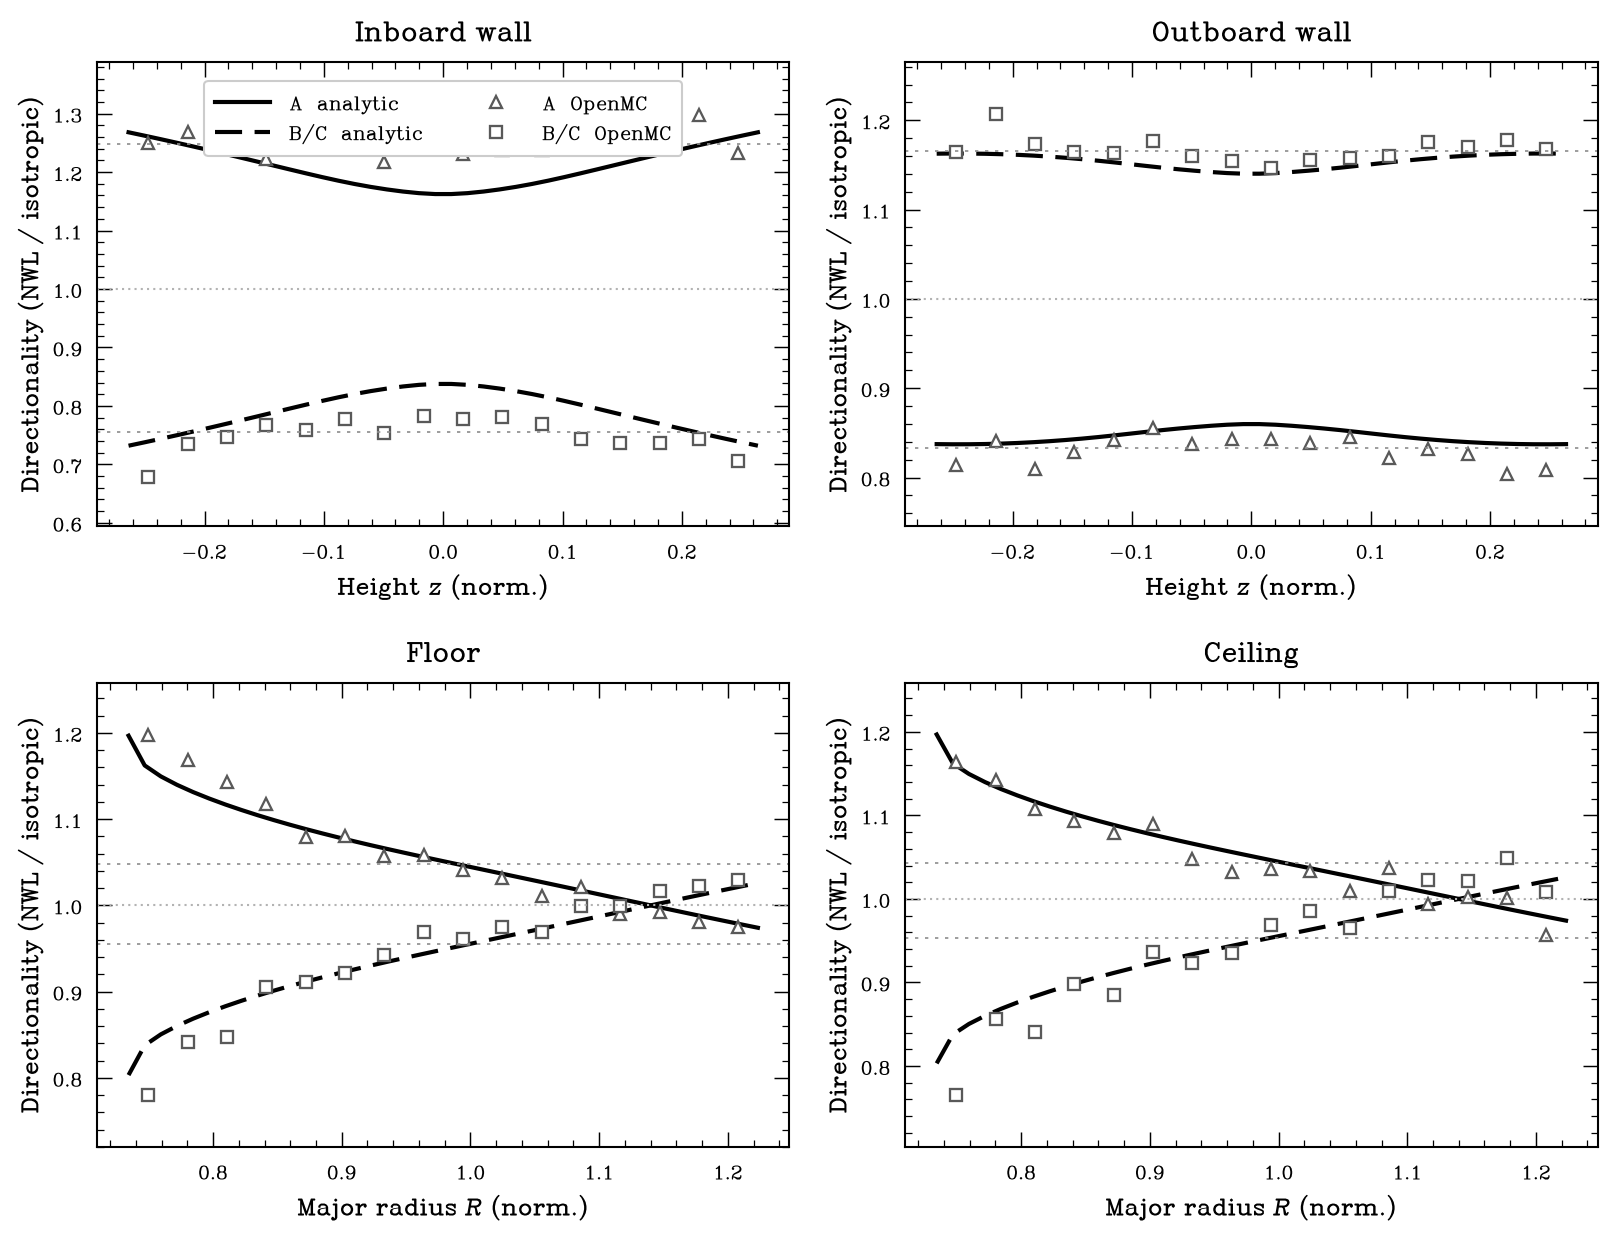
\includegraphics[width=\linewidth]{quasr59509_directionality.png}
\caption{Free-streaming directionality $A/\iso$ (mode A) and $B/\iso$ (mode B/C) around
each wall of the square torus for the real QUASR QA equilibrium ($\epseff\approx0.43$):
the analytic point-patch flux integral (curves) and the OpenMC ray-traced source
(markers). The outboard, floor, and ceiling walls overlay; the inboard wall tracks the
poloidal shape with the $4$--$6\%$ offset analyzed in Sec.~\ref{sec:pointpatch}. Per-panel
vertical scales because the walls differ by an order of magnitude in poloidal curvature.}
\label{fig:quasr}
\end{figure}

\section{The point-patch limit of the analytic method}
\label{sec:pointpatch}

The inboard residual is small but coherent, and its cause is worth establishing because it
maps the boundary between the two methods. We first eliminate the Monte-Carlo source as
the cause, then reproduce the effect by direct construction.

\paragraph{By elimination.}
The residual is not the direction sampler, which reproduces the kernels exactly
(Sec.~\ref{sec:sampler}). It is not the analytic quadrature, which matches
\texttt{anarr\'ima} to $10^{-12}$. It is not the visibility model: using the true
shaped-loop $N>0$ sub-arcs intersected with the inner-cylinder occlusion---rather than a
mean-radius, uncapped arc---removes an unrelated outboard error but leaves the inboard
value unchanged. It is not the field model, because the analytic and Monte-Carlo
evaluations call the identical $\Bhat$, which cannot by itself open a gap between them. And
it is not a near-field effect of the wall proximity: moving the wall outward from a gap of
$0.4\,a$ to $0.7\,a$ leaves the offset unchanged ($0.036\to0.034$). What does change it is
the plasma shaping---the gentle toy agrees on the inboard wall to $1.8\%$, the strongly
shaped QA does not---so the effect is a coupling of the source shaping to the wall
geometry that the two methods treat differently.

\paragraph{By construction.}
The one geometric approximation in the analytic NWL is that each wall patch is a point:
the emission kernel is evaluated along the single line of sight from the source to the
patch centre, whereas a patch on a curved wall subtends a finite solid angle over which
the kernel varies, and the ray-traced Monte-Carlo resolves it. To exhibit this in
isolation we strip the problem to a single shaped filament with a tunable shaping
amplitude $s$, emitting the kernel about a purely toroidal field onto bare inner and outer
cylinders, and evaluate the wall directionality two ways: the analytic point-patch flux
integral, and an exact ray/surface intersection of the same sampled births (the transport,
with no point-patch approximation). Here the sampler, field, and occlusion are all
trivially correct, so the shaping amplitude is the only variable.

The result (Fig.~\ref{fig:barecyl}) is decisive. At $s=0$, an axisymmetric source, the
point-patch integral is \emph{exact}: the analytic and ray-traced directionalities agree
to $0.002$, the Monte-Carlo statistical floor. As $s$ increases the two diverge, with the
discrepancy growing as $s^2$, and it grows about three times faster on the convex inner
cylinder (the inboard analogue) than on the concave outer cylinder (the outboard
analogue), reaching $\sim10\%$ on the inner wall at the strongest shaping. This reproduces,
in a controlled single-filament setting, both the inboard-specific location and the
shaping scaling of the residual seen on the full QA equilibrium, and it identifies the
cause unambiguously as the point-patch treatment of the flux integral on a strongly curved
wall---a property of the analytic method, with the geometry-exact, sampler-exact
Monte-Carlo source as the reference. It is precisely the kind of strongly shaped,
strongly curved regime that motivates a transport calculation in the first place.

\begin{figure}[t]
\centering
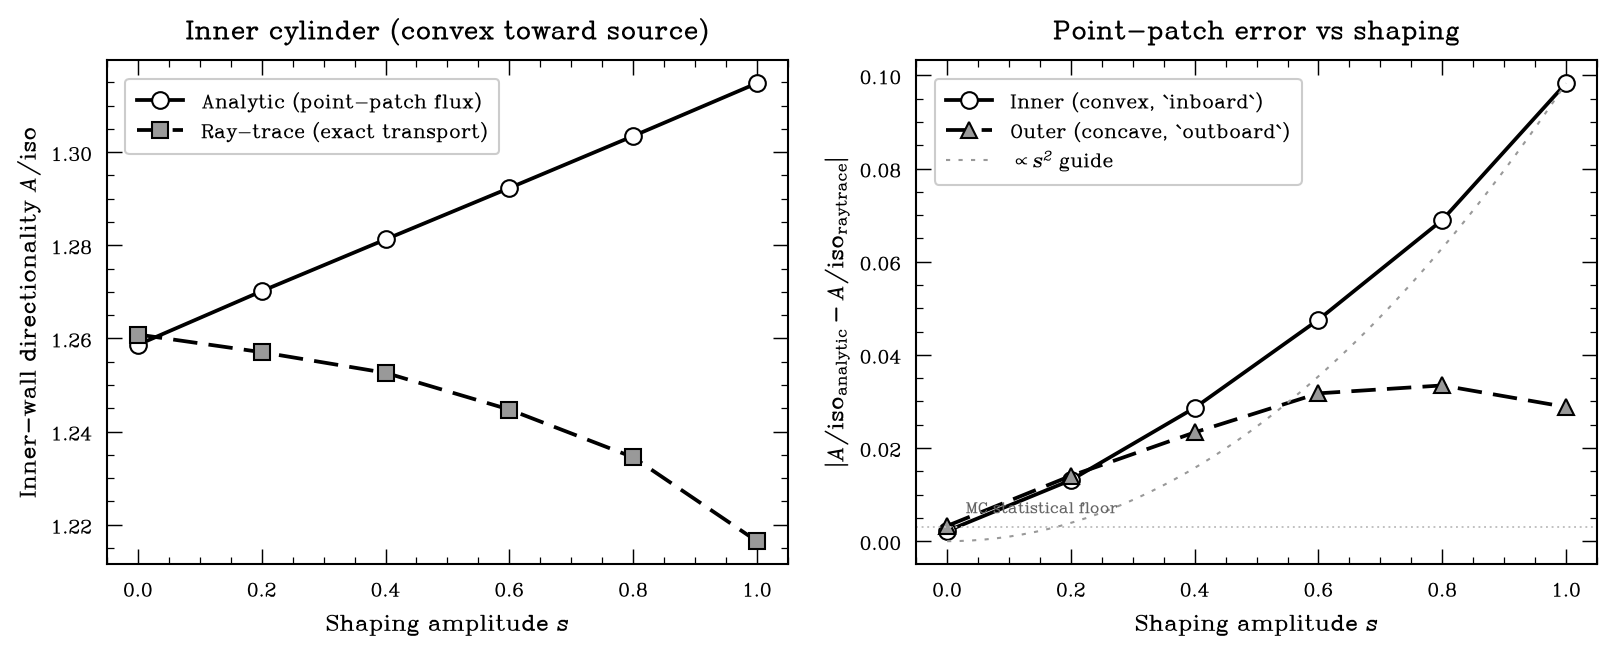
\includegraphics[width=\linewidth]{bare_cylinder_demo.png}
\caption{Single-filament demonstration that the inboard residual is the analytic
point-patch limit. Left: inner-wall directionality $A/\iso$ from the analytic point-patch
flux integral and from exact ray-tracing of the same births, versus the shaping amplitude
$s$; coincident for an axisymmetric source ($s=0$) and diverging as $s$ grows. Right: the
analytic$\leftrightarrow$ray-trace discrepancy versus $s$ for the convex inner (inboard)
and concave outer (outboard) cylinders, with an $s^2$ guide; zero to Monte-Carlo
statistics without shaping, growing quadratically with shaping and largest on the convex
inner wall.}
\label{fig:barecyl}
\end{figure}

\section{Toward transport on a realistic wall}
\label{sec:outlook}

The free-streaming cross-check certifies the source; the reason to have a Monte-Carlo
source is what the analytic method cannot do. Two extensions follow directly and change no
part of the sampler. The first is geometry: the same pre-sampled or compiled source drives
a run on a CAD first wall imported through DAGMC~\cite{dagmc} or on a CSG blanket model,
so the polarized load is evaluated on the true toroidal-field-coil-limited wall shape
rather than an idealized torus, and on the strongly shaped boundaries where the analytic
expansion is out of its band. The second is physics: replacing the void interior and
vacuum walls with a first wall, breeder, and shield turns the first-flight NWL into the
transported neutron flux and heating that set the tritium breeding ratio and the blanket
lifetime. The polarized angular emission enters that calculation only through the source;
everything downstream is standard neutron transport, so the anisotropy is carried into the
volumetric loads without approximation. These runs are most naturally performed where
DAGMC and OpenMC install together against a common cross-section library; we report them
separately.

Two limitations bound the present results. The birth model is filamentary or
flux-surface-weighted rather than a self-consistent fusion reactivity profile, and the
field is a model flux-surface-tangent field rather than a VMEC solution; both are shared
exactly between the two methods, so they do not affect the cross-validation, but a
physical run should replace them with a reactivity-weighted volumetric source and the
equilibrium field. Neither touches the sampler, which is the object this paper verifies.

\section{Summary}
\label{sec:summary}

We have built and verified a Monte-Carlo spin-polarized fusion neutron source for OpenMC.
The emission kernel separates cleanly into a birth-direction distribution, sampled exactly
by stratification over the two polarized angular shapes with inverse-CDF draws
cross-checked against rejection, and a scalar rate factor applied to the source strength;
the local-to-global rotation is degeneracy-free and bias-free. The sampler reproduces the
normalized polarized kernels to $0.3\%$ with unit mean, independent of any geometry. Run
as a free-streaming source on a shared wall, it reproduces the companion analytic method's
NWL to $\le1.8\%$ on a gentle QA boundary on all walls, and to $\le1.8\%$ on three walls of
a real, strongly shaped published QA equilibrium mined from the QUASR database. The one
larger residual, $4$--$6\%$ on the strongly curved inboard wall of the strongly shaped
case, we have shown---by systematic elimination and by a single-filament construction that
is exact for an axisymmetric source and grows as the square of the shaping amplitude---to
be a limit of the analytic point-patch flux integral rather than a defect of the
Monte-Carlo source. The two methods thus partition the problem cleanly: the closed,
differentiable analytic form where the boundary is weakly shaped and gradients drive
optimization, and the present source where the shaping is strong or where the neutron
transport on a realistic wall---the calculation the free-streaming methods cannot
perform---is what a reactor design actually needs.

\begin{thebibliography}{99}

\bibitem{schwartz2025}
J.~Schwartz \emph{et al.}, Neutron wall loading for spin-polarized fusion in axisymmetric
geometries, 2025.

\bibitem{lion2022}
J.~Lion \emph{et al.}, A deterministic method for stellarator neutron wall loading, 2022.

\bibitem{parisi2024}
J.~F.~Parisi \emph{et al.}, Spin-polarized fusion in magnetic confinement, 2024.

\bibitem{kulsrud1982}
R.~M.~Kulsrud, H.~P.~Furth, E.~J.~Valeo, and M.~Goldhaber,
Fusion reactor plasmas with polarized nuclei,
\emph{Phys. Rev. Lett.} \textbf{49}, 1248 (1982).

\bibitem{landreman2022}
M.~Landreman and E.~Paul, Magnetic fields with precise quasisymmetry for plasma
confinement, \emph{Phys. Rev. Lett.} \textbf{128}, 035001 (2022).

\bibitem{romano2015}
P.~K.~Romano, N.~E.~Horelik, B.~R.~Herman, A.~G.~Nelson, B.~Forget, and K.~Smith,
OpenMC: A state-of-the-art Monte Carlo code for research and development,
\emph{Ann. Nucl. Energy} \textbf{82}, 90 (2015).

\bibitem{dagmc}
P.~C.~Shriwise, A.~Davis, L.~J.~Jacobson, and P.~P.~H.~Wilson,
Particle tracking acceleration on CAD geometries in DAGMC, 2017.

\bibitem{quasr}
A.~Giuliani \emph{et al.}, QUASR: a database of quasisymmetric stellarators and their
coils, Flatiron Institute; \url{https://quasr.flatironinstitute.org}.

\end{thebibliography}

\end{document}
